\documentclass[12pt, oneside]{article} 
\usepackage{amsmath, amsthm, amssymb, calrsfs, wasysym, verbatim, bbm, color, graphicx, geometry, fancyhdr, url, multirow, hyperref, titlesec, tabularx, spreadtab, pgf-pie, eurosym}
\usepackage[italian]{babel}
\usepackage{colortbl}

\geometry{tmargin=.75in, bmargin=.75in, lmargin=.75in, rmargin = .75in}

% Creo subsubsubsection
\titleclass{\subsubsubsection}{straight}[\subsection]

\newcounter{subsubsubsection}[subsubsection]
\renewcommand\thesubsubsubsection{\thesubsubsection.\arabic{subsubsubsection}}
\renewcommand\theparagraph{\thesubsubsubsection.\arabic{paragraph}} % optional; useful if paragraphs are to be numbered

\titleformat{\subsubsubsection}
  {\normalfont\normalsize\bfseries}{\thesubsubsubsection}{1em}{}
\titlespacing*{\subsubsubsection}
{0pt}{3.25ex plus 1ex minus .2ex}{1.5ex plus .2ex}

\makeatletter
\renewcommand\paragraph{\@startsection{paragraph}{5}{\z@}%
  {3.25ex \@plus1ex \@minus.2ex}%
  {-1em}%
  {\normalfont\normalsize\bfseries}}
\renewcommand\subparagraph{\@startsection{subparagraph}{6}{\parindent}%
  {3.25ex \@plus1ex \@minus .2ex}%
  {-1em}%
  {\normalfont\normalsize\bfseries}}
\def\toclevel@subsubsubsection{4}
\def\toclevel@paragraph{5}
\def\toclevel@paragraph{6}
\def\l@subsubsubsection{\@dottedtocline{4}{7em}{4em}}
\def\l@paragraph{\@dottedtocline{5}{10em}{5em}}
\def\l@subparagraph{\@dottedtocline{6}{14em}{6em}}
\makeatother

\setcounter{secnumdepth}{4}
\setcounter{tocdepth}{4}
% Fine creazione subsubsubsection

\author{RAMtastic6}

%Intestazione
\pagestyle{fancy}
\fancyhf{}
\fancyhead[R]{Gruppo 14 RAMtastic6\\ramtastic6@gmail.com}
\fancyfoot[C]{\thepage}

% Linea intestazione
\renewcommand{\headrulewidth}{0pt} 

% Intestazione documento
\begin{document}
% Salta la prima pagina per l'intestazione
\thispagestyle{empty}
\title{\textit{Piano di Qualifica}_G}
\maketitle
\begin{figure}[h]
  \centering
  
\includegraphics[scale=0.3]{logo.png}
\end{figure}
\begin{center}
    email: ramtastic6@gmail.com
\end{center}

% Informazioni sul documento
\section*{Informazioni sul documento}
\begin{tabular}{ll}
Versione: & 0.0.2 \\
Redattori: & Riccardo Z. \\
Verificatori: & \\ 
Destinatari: & T. Vardanega, R. Cardin, \textit{Imola Informatica}_G \\
Uso: & Esterno
\end{tabular}
\newpage

% Registro dei cambiamenti
\section*{Registro dei Cambiamenti - Changelog}
\begin{tabular}{|c|c|c|p{3cm}|p{6cm}|}
\hline
\textbf{Versione} & \textbf{Data} & \textbf{Autore} & \textbf{Verificatore} & \textbf{Dettaglio} \\
\hline
v.0.0.3 & 13-03-2024 & Riccardo Z. & N/A & Stesura delle prime versioni della sezione "\textit{Test}_Ging" e della sezione "Checklist"\\
\hline
v.0.0.2 & 12-03-2024 & Riccardo Z. & N/A & Stesura delle prime versioni delle sottosezioni di "Obiettivi di qualita": "Documentazione" e "Sviluppo"\\
\hline
v.0.0.1 & 11-03-2024 & Riccardo Z. & N/A & Prima versione, identificazione delle sezioni principali, stesura della sezione 1 "Introduzione", della sezione introduttiva di "\textit{Qualità di processo}_G" e di "\textit{Qualità di prodotto}_G" e della sottosezione "\textit{Fornitura}_G" \\
\hline
\end{tabular}
\newpage


% Sommario
\tableofcontents
\newpage
\section{Introduzione}
\subsection{Scopo del documento}
Il presente documento si propone di definire le metriche e le metodologie di controllo e misurazione necessarie per garantire la qualità del prodotto e del processo. In particolare, le metriche di valutazione del prodotto sono correlate ai requisiti e alle aspettative del fornitore.
Il Piano di Qualifica è concepito per essere dinamico ed incrementale, in particolar modo per quanto riguarda le metriche descritte e mira a fornire una valutazione il più obiettiva possibile di ciò che è stato realizzato.\\
Le procedure del Way of Working devono essere costantemente osservate e migliorate, al fine di garantire che il prodotto soddisfi le aspettative del cliente e mantenga gli standard di qualità richiesti. Eventuali termini tecnici sono definiti all'interno del documento "Glossario Tecnico".

\subsection{Riferimenti}
\subsubsection{Riferimenti normativi}
\begin{enumerate}
    \item Norme di Progetto
    \item Presentazione del capitolato d'appalto C3 - Progetto Easy Meal: \\ 
    \url{https://www.math.unipd.it/~tullio/IS-1/2023/Progetto/C3.pdf}
    \item Regolamento del progetto didattico: \\ 
    \url{https://www.math.unipd.it/~tullio/IS-1/2023/Dispense/PD2.pdf}
\end{enumerate}
\subsubsection{Riferimenti informativi}
\label{sec:rif_inf}
\begin{enumerate}
    \item Lezione \emph{"Progettazione software (T6)"} del corso di Ingegneria del software: \\
    \url{https://www.math.unipd.it/~tullio/IS-1/2023/Dispense/T6.pdf}
    \item Lezione \emph{"Qualità del software (T7)"} del corso di Ingegneria del software: \\
    \url{https://www.math.unipd.it/~tullio/IS-1/2023/Dispense/T7.pdf}
    \item Lezione \emph{"Qualità di processo (T8)"} del corso di Ingegneria del software: \\
    \url{https://www.math.unipd.it/~tullio/IS-1/2023/Dispense/T8.pdf}
    \item Lezione \emph{"Verifica e validazione: introduzione (T9)"} del corso di Ingegneria del software: \\
    \url{https://www.math.unipd.it/~tullio/IS-1/2023/Dispense/T9.pdf}
    \item Lezione \emph{"Verifica e validazione: analisi statica (T10)"} del corso di Ingegneria del software: \\
    \url{https://www.math.unipd.it/~tullio/IS-1/2023/Dispense/T10.pdf}
    \item Lezione \emph{"Verifica e validazione: analisi dinamica (T11)"} del corso di Ingegneria del software: \\
    \url{https://www.math.unipd.it/~tullio/IS-1/2023/Dispense/T11.pdf}
     \item Documento \emph{"Dichiarazione impegni v1.2"}: \\ \url{https://github.com/RAMtastic6/Project14/blob/main/documenti/CANDIDATURA/documento_impegni_v1.2.pdf}
     \item Metriche di progetto (\emph{Earned Value Analysis}):\\
     \url{https://it.wikipedia.org/wiki/Metriche_di_progetto}
\end{enumerate}
\subsection{Codifica delle metriche}
In questa sottosezione verranno definite le metriche che utilizzeremo, utilizzando un codice standardizzato.

Una metrica è identificata dal seguente formato di codice:
\[
\text{M[Tipo][Id]-[Acronimo]}
\]

Dove:
\begin{itemize}
    \item \textbf{M} sta per "Metrica"
    \item \textbf{Tipo} può essere PC (per un processo) o PD (per un prodotto)
    \item \textbf{Id} rappresenta un identificativo all'interno di una metrica di un certo tipo
    \item \textbf{Acronimo} indica l'acronimo del nome della metrica utilizzata
\end{itemize}

Per ciascuna metrica verranno fornite descrizioni, valori accettabili e valori preferibili.
\newpage
\input{sections/obiettivi_qualità}
\newpage


\section{Testing}
In questa sezione vengono esplorate le metodologie di testing e la loro specifica. L'obiettivo è quello di seguire il Modello a V in cui ad ogni fase di sviluppo corrisponde una tipologia di test da eseguire.\\
I test si dividono in:
\begin{itemize}
    \item \textbf{Test di unità}:\\
    vengono eseguiti sulle unità più semplici del codice. Viene fatta corrispondere all'attività di codifica (implementation).
    \item \textbf{Test di integrazione}:\\
    vengono eseguiti per verificare la corretta integrazione tra le diverse unità software. Viene fatta corrispondere all'attività di progettazione.
    \item \textbf{Test di sistema}:\\
    verificano il corretto funzionamento dell'intero sistema e, in particolare, che tutti i requisiti individuati siano soddisfatti. Viene fatta corrispondere all'attività di Analisi Dei Requisiti. 
    \item \textbf{Test di accettazione}:\\
    verificano, alla presenza del committente, che il prodotto finale soddisfi tutti i requisiti. Se superati, si può procedere al rilascio dello stesso.
\end{itemize}
\subsection{Test di sistema}
I test di sistema sono una fase del processo di testing il cui scopo è quello di verificare che il sistema software rispetti i requisiti specificati nel documento "Analisi Dei Requisiti".
Di seguito verranno elencati i vari test, i quali avranno un codice identificativo, una descrizione, il requisito a cui fa riferimento e lo stato del test.
%\begin{table}[htbp]
    %\centering
    \begin{longtable}{|>{\centering\arraybackslash}p{1.5cm}|p{9.8cm}|p{2cm}|p{3.5cm}|}
    \hline
    \rowcolor{gray!30}
    \textbf{Codice} & \textbf{Descrizione} & \textbf{Requisito} & \textbf{Stato} \\
    \hline
    \rowcolor{gray!10}
    \textbf{TS-01} & Verificare che l'utente base possa visualizzare i pasti ordinabili & ROF 1 & Non implementato \\
    \hline
    \rowcolor{gray!10}
    \textbf{TS-04} & Verificare che il sistema possa inviare una notifica se l'utente base sta aggiungendo un piatto che contiene elementi a cui è allergico/intollerante & ROF 2 & Non implementato \\ 
    \hline 
    \rowcolor{gray!10}
    \textbf{TS-05} & Verificare che l'utente possa visualizzare i pasti con i loro ingredienti e che possa modificarli, aggiungendo o togliendo ingredienti & ROF 3 & Non implementato \\ 
    \hline
    \rowcolor{gray!10}
    \textbf{TS-06} & Verificare che l'utente base possa essere in grado di visualizzare il riepilogo di quanto ordinato e che possa confermare oppure cancellare l'ordine & ROF 4 & Non implementato \\ 
    \hline
    \rowcolor{gray!10}
    \textbf{TS-07} & Verificare che il sistema possa inviare una notifica (push) di prenotazione effettuata ai ristoranti & RDF 5 & Non implementato \\ 
    \hline
    \rowcolor{gray!10}
    \textbf{TS-08} & Verificare che l'utente possa inserire le informazioni (data, orario, persone, nomi utenti) per effettuare una prenotazione & ROF 6 & Non implementato \\
    \hline
    \rowcolor{gray!10}
    \textbf{TS-09} & Verificare che il sistema possa inviare una notifica (push) agli amministratori per comunicare la richiesta di prenotazione, che può accettare o rifiutare & RDF 7 & Non implementato \\
    \hline
    \rowcolor{gray!10}
    \textbf{TS-10} & Verificare che l'utente possa essere in grado di cancellare la prenotazione & ROF 8 & Non implementato \\ 
    \hline
    \rowcolor{gray!10}
    \textbf{TS-11} & Verificare che il sistema possa negare la prenotazione se il ristorante non possiede abbastanza posti o tavoli & ROF 9 & Non implementato \\ 
    \hline
    \rowcolor{gray!10}
    \textbf{TS-12} & Verificare che l'utente base possa visualizzare una lista di ristoranti filtrata per nome, data, luogo o tipologia cucina & ROF 10 & Non implementato \\ 
    \hline
    \rowcolor{gray!10}
    \textbf{TS-13} & Verificare che l'utente base possa selezionare un ristorante & ROF 11 & Non implementato \\ 
    \hline
    \rowcolor{gray!10}
    \textbf{TS-14} & Verificare che l'amministratore possa visualizzare una lista di prenotazioni in attesa & ROF 12 & Non implementato \\
    \hline
    \rowcolor{gray!10}
    \textbf{TS-15} & Verificare che l'amministratore possa selezionare una specifica richiesta di prenotazione dalla lista visualizzata & ROF 13 & Non implementato \\ 
    \hline
    \rowcolor{gray!10}
    \textbf{TS-16} & Verificare che l'amministratore possa accettare la richiesta di prenotazione selezionata & ROF 14 & Non implementato \\ 
    \hline
    \rowcolor{gray!10}
    \textbf{TS-17} & Verificare che il sistema possa aggiungere la prenotazione nell'area "prenotazioni" dell'utente & ROF 15 & Non implementato \\
    \hline
    \rowcolor{gray!10}
    \textbf{TS-18} & Verificare che il sistema possa notificare gli utenti coinvolti (nel caso di prenotazione collaborativa) dell'accettazione della prenotazione & ROF 16 & Non implementato \\ 
    \hline
    \rowcolor{gray!10}
    \textbf{TS-19} & Verificare che il sistema possa fornire un'interfaccia per consentire all'amministratore di verificare la disponibilità di posti in base alle specifiche della prenotazione selezionata & ROF 17 & Non implementato \\ 
    \hline
    \rowcolor{gray!10}
    \textbf{TS-20} & Verificare che il sistema possa ridurre il numero di posti disponibili in base alle specifiche della prenotazione accettata & ROF 18 & Non implementato \\ 
    \hline
    \rowcolor{gray!10}
    \textbf{TS-21} & Verificare che l'amministratore possa rifiutare la richiesta di prenotazione selezionata & ROF 19 & Non implementato \\ 
    \hline
    \rowcolor{gray!10}
    \textbf{TS-22} & Verificare che il sistema possa notificare gli utenti coinvolti (nel caso di prenotazione collaborativa) del rifiuto della prenotazione & ROF 20 & Non implementato \\ 
    \hline
    \rowcolor{gray!10}
    \textbf{TS-24} & Verificare che il sistema possa creare un canale di comunicazione tra l'utente e l'amministratore del ristorante quando l'utente lo richiede & ROF 21 & Non implementato \\
    \hline
    \rowcolor{gray!10}
    \textbf{TS-25} & Verificare che l'utente e l'amministratore possano scambiarsi messaggi in modo bidirezionale tramite l'interfaccia di comunicazione & ROF 22 & Non implementato \\ 
    \hline 
    \rowcolor{gray!10}
    \textbf{TS-26} & Verificare che durante la comunicazione, il sistema possa inviare notifiche push per informare l'utente e l'amministratore dei nuovi messaggi ricevuti & ROF 23 & Non implementato \\ 
    \hline
    \rowcolor{gray!10}
    \textbf{TS-27} & Verificare che la cancellazione della prenotazione possa essere effettuata con al massimo un giorno di anticipo rispetto alla data della prenotazione & ROF 24 & Non implementato \\
    \hline
    \rowcolor{gray!10}
    \textbf{TS-31} & Verificare che il sistema permetta di pagare il conto in base alla modalità scelta (divisione equa, divisione proporzionale) da chi ha creato la ordinazione collaborativa & ROF 25 & Non implementato \\
    \hline
    \rowcolor{gray!10}
    \textbf{TS-32} & Verificare che l'utente base possa pagare tutto il conto se nessun utente ha pagato & ROF 26 & Non implementato \\
    \hline
    \rowcolor{gray!10}
    \textbf{TS-33} & Verificare che l'amministratore possa modificare il menu' del proprio ristorante, aggiungendo, rimuovendo pietanze e modificando le informazioni del singolo piatto (nome, ingredienti e prezzo) & ROF 27 & Non implementato \\
    \hline
    \rowcolor{gray!10}
    \textbf{TS-34} & Verificare che la modifica del menù da parte dell'amministratore non causi problemi di sincronizzazione nella visualizzazione, ricerca del menu' e nell'ordinazione da parte dell'utente base & RDF 28 & Non implementato \\ 
    \hline
    \rowcolor{gray!10}
    \textbf{TS-35} & Verificare che l'utente base possa inserire un coupon prima di pagare il conto, che, se applicato, deve far ricalcolare al sistema il prezzo del conto & RDF 29 & Non implementato \\ 
    \hline
    \rowcolor{gray!10}
    \textbf{TS-36} & Verificare che l'amministratore possa consultare le prenotazioni associate al proprio ristorante & ROF 30 & Non implementato \\ 
    \hline
    \rowcolor{gray!10}
    \textbf{TS-38} & Verificare che l'amministratore possa visualizzare i dettagli completi di una specifica prenotazione & ROF 31 & Non implementato \\ 
    \hline
    \rowcolor{gray!10}
    \textbf{TS-39} & Verificare che l'amministratore possa visualizzare lo stato delle ordinazioni associate alla prenotazione & ROF 32 & Non implementato \\ 
    \hline
    \rowcolor{gray!10}
    \textbf{TS-40} & Verificare che il sistema possa fornire all'amministratore la possibilità di visualizzare la lista totale degli ingredienti inclusi nella prenotazione & RDF 33 & Non implementato \\ 
    \hline
    \rowcolor{gray!10}
    \textbf{TS-41} & Verificare che il sistema possa consentire all'amministratore di visualizzare tutti gli ordini confermati per il ristorante selezionato & ROF 34 & Non implementato \\ 
    \hline
    \rowcolor{gray!10}
    \textbf{TS-42} & Verificare che il sistema possa permettere di annullare l'ordinazione collaborativa nel tempo utile per farlo & ROF 35 & Non implementato \\
    \hline
    \rowcolor{gray!10}
    \textbf{TS-43} & Verificare che il sistema invii una notifica a tutti gli utenti associati alla prenotazione la cui ordinazione collaborativa è stata annullata & RDF 36 & Non implementato \\ 
    \hline
    \rowcolor{gray!10}
    \textbf{TS-44} & Verificare che il sistema fornisca un'interfaccia per consentire agli utenti non autenticati di registrarsi come utenti base & ROF 37 & Non implementato \\ 
    \hline
    \rowcolor{gray!10}
    \textbf{TS-45} & Verificare che l'utente/l'amministratore possa inserire le sue informazioni personali durante la registrazione come nome, cognome, email, password ed eventuali intolleranze & ROF 38 & Non implementato \\
    \hline
    \rowcolor{gray!10}
    \textbf{TS-46} & Verificare che l'utente/l'amministratore possa confermare di volersi registrare con le informazioni fornite prima di completare la registrazione & ROF 39 & Non implementato \\ 
    \hline
    \rowcolor{gray!10}
    \textbf{TS-47} & Verificare che il sistema gestisca correttamente gli errori nell'inserimento delle informazioni durante la registrazione & ROF 40 & Non implementato \\ 
    \hline
    \rowcolor{gray!10}
    \textbf{TS-48} & Verificare che l'utente base e l'amministratore possano visualizzare il menu' del ristorante selezionato & ROF 41 & Non implementato \\ 
    \hline
    \rowcolor{gray!10}
    \textbf{TS-49} & Verificare che l'amministratore possa modificare le informazioni del proprio ristorante (nome, indirizzo, orari, coperti e tipologia di cucina) & ROF 42 & Non implementato \\
    \hline
    \rowcolor{gray!10}
    \textbf{TS-50} & Verificare che la modifica delle informazioni del ristorante da parte dell'amministratore non causi problemi di sincronizzazione nella visualizzazione, ricerca del ristorante e nell'ordinazione da parte dell'utente base & RDF 43 & Non implementato \\ 
    \hline
    \rowcolor{gray!10}
    \textbf{TS-51} & Verificare che l'utente autenticato possa visualizzare una lista con le prenotazioni passate e future & ROF 44 & Non implementato \\ 
    \hline
    \rowcolor{gray!10}
    \textbf{TS-52} & Verificare che l'utente autenticato possa rilasciare una recensione (con anche una votazione di gradimento tramite stelle) sui ristoranti nei quali ha effettuato almeno una prenotazione & ROF 45 & Non implementato \\ 
    \hline
    \rowcolor{gray!10}
    \textbf{TS-53} & Verificare che l'utente autenticato possa visualizzare gli ordini di un tavolo & ROF 46 & Non implementato \\ 
    \hline
    \rowcolor{gray!10}
    \textbf{TS-54} & Verificare che l'utente autenticato possa visualizzare le recensioni rilasciate ed eventualmente eliminarle & ROF 47 & Non implementato \\ 
    \hline
    \rowcolor{gray!10}
    \textbf{TS-55} & Verificare che l'utente generico possa visualizzare le recensioni di un ristorante e visualizzare per ognuna di essa le relative informazioni & ROF 48 & Non implementato \\ 
    \hline
    \rowcolor{gray!10}
    \textbf{TS-56} & Verificare che l'amministratore possa inserire le informazioni del ristorante di cui è amministratore & ROF 49 & Non implementato \\
    \hline
    \rowcolor{gray!10}
    \textbf{TS-57} & Verificare che l'utente/l'amministratore possa inserire la propria email e la password durante la fase di login & ROF 50 & Non implementato \\ 
    \hline
    \rowcolor{gray!10}
    \textbf{TS-58} & Verificare che il sistema verifichi che le informazioni inserite nel login corrispondano ad un account esistente nel sistema & ROF 51 & Non implementato \\ 
    \hline
    \rowcolor{gray!10}
    \textbf{TS-59} & Verificare che il sistema predisponga in fase di login di un'opzione per il recupero della password & ROF 52 & Non implementato \\ 
    \hline
    \rowcolor{gray!10}
    \textbf{TS-60} & Verificare che l'utente non autenticato possa inserire la propria email durante il processo di recupero password & ROF 53 & Non implementato \\ 
    \hline
    \rowcolor{gray!10}
    \textbf{TS-61} & Verificare che, se l'email inserita dall'utente corrisponde a un account nel sistema, il sistema invii un'email contenente un link per il recupero della password & ROF 54 & Non implementato \\
    \hline
    \rowcolor{gray!10}
    \textbf{TS-62} & Verificare che, se l'email inserita dall'utente non corrisponde a un account nel sistema, il sistema lo mostri a schermo & ROF 55 & Non implementato \\ 
    \hline
    \rowcolor{gray!10}
    \textbf{TS-63} & Verificare che l'utente possa accedere a una sezione dedicata tramite il link fornito nell'email di recupero password & ROF 56 & Non implementato \\ 
    \hline
    \rowcolor{gray!10}
    \textbf{TS-64} & Verificare che il sistema mostri una lista di prenotazioni, ognuna con le seguenti informazioni:
    Nome del ristorante, Data, Ora, Stato della prenotazione (se è ancora attiva o già completata) e Numero di persone coinvolte & ROF 57 & Non implementato \\
    \hline
    \rowcolor{gray!10}
    \textbf{TS-65} & Verificare che il sistema ordini la lista delle prenotazioni per data della prenotazione & RDF 58 & Non implementato \\ 
    \hline
    \rowcolor{gray!10}
    \textbf{TS-67} & Verificare che l'utente possa inserire le proprie allergie/intolleranze, se presenti, durante la modifica del profilo & ROF 59 & Non implementato \\ 
    \hline
    \rowcolor{gray!10}
    \textbf{TS-69} & Verificare che l'utente autenticato e l'amministratore possano inserire nome,cognome,mail e password nell'area di modifica delle proprie informazioni & ROF 60 & Non implementato \\ 
    \hline
    \rowcolor{gray!10}
    \textbf{TS-70} & Verificare che il sistema verifichi che l'email inserita dall'utente autenticato/amministratore sia valida e non sia già presente nel sistema & ROF 61 & Non implementato \\ 
    \hline
    \rowcolor{gray!10}
    \textbf{TS-71} & Verificare che l'utente base autenticato possa accedere alla funzionalità di ordinazione di un piatto & ROF 62 & Non implementato \\
    \hline
    \rowcolor{gray!10}
    \textbf{TS-73} & Verificare che il sistema consenta all'utente di visualizzare, aggiungere e togliere ingredienti del piatto selezionato & ROF 63 & Non implementato \\
    \hline
    \rowcolor{gray!10}
    \textbf{TS-74} & Verificare che l'amministratore possa visualizzare le recensioni del proprio ristorante & ROF 64 & Non implementato \\ 
    \hline
    \rowcolor{gray!10}
    \textbf{TS-75} & Verificare che l'amministratore possa rispondere alle recensioni del proprio ristorante & ROF 65 & Non implementato \\ 
    \hline
    \rowcolor{gray!10}
    \textbf{TS-76} & Verificare che l'utente possa visualizzare le risposte alla propria recensione & ROF 66 & Non implementato \\
    \hline
    \rowcolor{gray!10}
    \textbf{TS-77} & Verificare che il sistema consenta di modificare l'ordine ad un utente prima della scadenza del tempo previsto, inserendo piatti, modificando ingredienti e quantità delle pietanze ordinate & ROF 67 & Non implementato \\ 
    \hline
    \rowcolor{gray!10}
    \textbf{TS-78} & Verificare che il sistema permetta di far visualizzare all'amministratore il dettaglio degli ingredienti necessari per ogni giornata & RDF 68 & Non implementato \\ 
    \hline
    \rowcolor{gray!10}
    \textbf{TS-89} & Verificare che il sistema consenta all'utente autenticato di selezionare l'opzione di logout & ROF 69 & Non implementato \\
    \hline
    \rowcolor{gray!10}
    \textbf{TS-80} & Verificare che, dopo che l'utente ha selezionato l'opzione di logout, il sistema richieda una conferma esplicita dall'utente prima di procedere con la disconnessione & ROF 70 & Non implementato \\ 
    \hline
    \rowcolor{gray!10}
    \textbf{TS-81} & Verificare che, dopo aver terminato la sessione dell'utente, il sistema reindirizzi l'utente alla pagina di accesso o a una pagina di destinazione predefinita & ROF 71 & Non implementato \\ 
    \hline
    \rowcolor{gray!10}
    \textbf{TS-82} & Verificare che l'utente autenticato possa visualizzare le informazioni del suo profilo & ROF 72 & Non implementato \\ 
    \hline
    \rowcolor{gray!10}
    \textbf{TS-84} & Verificare che l'amministratore possa visualizzare tutte le chat aperte in precedenza da altri utenti& ROF 73 & Non implementato \\ 
    \hline
    \rowcolor{gray!10}
    \textbf{TS-85} & Verificare che l'amministratore possa rispondere alle chat con gli utenti & ROF 74 & Non implementato \\ 
    \hline
    \caption{Test di sistema} 
    \label{tab:test_sistema}
    \end{longtable}
    
%\end{table}
\newpage
\section{Checklist}
La verifica tramite analisi statica è preferibile che avvenga tramite ispezione anzichè walkthrough, per questo motivo sono definite delle liste di controllo aggiornate progressivamente dai verificatori che permettono rapidamente di analizzare gli errori più comuni e di verificare selettivamente.

\subsection{Documentazione}
\subsubsection{Struttura}
\begin{table}[h]
\centering
\begin{tabular}{|c|p{8cm}|}
\hline
\textbf{Errore} & \textbf{Descrizione} \\
\hline
Manca la caption per le tabelle o le immagini &  Ogni tabella o immagine deve possedere una caption\\
\hline
Sezione vuota & Le sezioni vuote devono essere eliminate\\
\hline
Parola non coincide con il glossario & Tale parola deve essere riportata con le stesse lettere maiuscole e minuscole rispetto al glossario eccetto la lettera iniziale\\
\hline
\end{tabular}
\caption{Checklist dei possibili errori nella struttura della documentazione}
\end{table}

\subsubsection{Errori ortografici}
\begin{table}[h]
\centering
\begin{tabular}{|c|p{8cm}|}
\hline
\textbf{Errore} & \textbf{Descrizione} \\
\hline
Errore di sintassi &  Errori di battitura o di distrazione devono essere rimossi\\
\hline
Errore di coniugazione & Gli errori di coniugazione devono essere rimossi\\
\hline
\end{tabular}
\caption{Checklist dei possibili errori ortografici nella documentazione}
\end{table}

\subsubsection{Analisi Dei Requisiti}
\begin{table}[h]
\centering
\begin{tabular}{|c|p{8cm}|}
\hline
\textbf{Errore} & \textbf{Descrizione} \\
\hline
Requisiti per un Caso d'Uso assenti &  Ad ogni Caso d'Uso deve corrispondere almeno un requisito\\
\hline
Diagrammi dei casi d'uso erronei & I diagrammi dei casi d'uso devono riportare la corretta numerazione e nomenclatura del caso d'uso stesso e riferirsi allo stesso modo ad altri casi d'uso\\
\hline
\end{tabular}
\caption{Checklist dei possibili errori per l'Analisi Dei Requisiti}
\end{table}
\newpage
\section{Cruscotto di valutazione della qualità}
\subsection{MPC01-EAC (Estimated at Completition)}
Dal grafico si può notare che l'EAC supera il valore accettabile di quest'ultimo. La causa di questa situazione si può ricondurre principalmente alla quasi assente divisione delle ore individuali e le ore produttive.
\subsection{MPC02-PV (Planned Value) e MPC04-EV (Earned Value)}
Dal grafico si può notare che le linee del PV e dell'EV sono molto vicine fra loro, ciò implica che il lavoro svolto è conforme a quello pianificato.
\subsection{MPC05-ETC (Estimated to Complete)}
Dal grafico si può notare che le linee dell'AC e dell'ETC nel corso dei vari periodi, mantengano un andamento costante. Di conseguenza si può affermare che il progetto stia mantenendo un ritmo regolare di avanzamento. 
\subsection{MPC08-BV (Budget Variance)}

\subsection{MPC09-RSI (Requirements stability index)}
\subsection{MPC14-IG (Indice Gulpeanse)}
\subsection{MPC15-NCR (Non Calculated Risk)}
\begin{figure}[H]
  \centering
  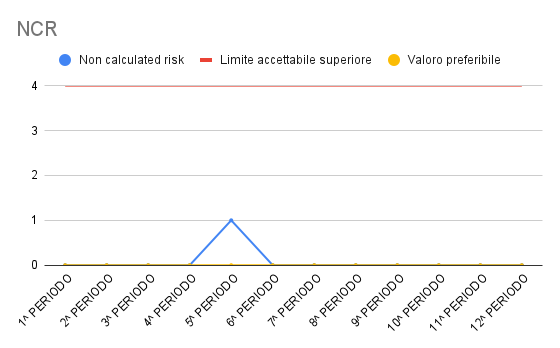
\includegraphics[width=0.7\linewidth]{grafici/NCR.png}
  \caption{Non Calculated Risk}
\end{figure}
Dal grafico si può notare che per la maggior parte del tempo non sono comparsi rischi non previsti. Solo nel quinto periodo si è emerso un rischio di cui non si era tenuto conto inizialmente, ovvero la sessione di esami, la quale ha portato via parecchio tempo ai vari membri del gruppo, rallentando di molto l'avanzamento del lavoro.
\subsection{MPC16-ET (Efficienza temporale)}

\newpage
\section{Valutazioni per il miglioramento}

In questa sezione viene riportata la valutazione generale sul lavoro con lo scopo di inserire osservazioni sui problemi presenti e sulle possibili correzioni da adottare come miglioramenti. 

\subsection{Valutazione sull’organizzazione}

\begin{table}[h]
\centering
\begin{tabular}{|p{3cm}|p{4cm}|c|p{5cm}|}
\hline
\rowcolor{gray!30}
\textbf{Problema} & \textbf{Descrizione} & \textbf{Gravità} & \textbf{Soluzione}\\
\hline
Tracciamento temporale & 
Il gruppo, nella fase iniziale del progetto, ha avuto delle difficoltà nel tracciamento delle ore per ogni attività del ruolo che copriva ogni membro & 
Media & 
Adottato l'uso di Jira per suddividere anche graficamente ogni attività in base allora sprint, con relativo tracciamento temporale per ogni task. \\
\hline
Meeting di gruppo &
Il gruppo, avendo diversi membri alle prese con esami arretrati o per esigenze lavorative, ha avuto qualvolta difficoltà nell'organizzare dei meeting di gruppo in cui fossero presenti tutti i partecipanti &
Bassa &
Con in passare del tempo dall'inizio del progetto si sono individuati le effettive fasce orarie in cui l'intero gruppo era disponibile per organizzare i meeting, salve imprevisti\\
\hline
Definizione casi d'uso &
Inizialmente è stato perso un po' di tempo per via della mancata definizione di un pattern da rispettare per trascrivere i casi d'uso nell'Analisi dei requisiti. &
Media &
In gruppo si è deciso un metodo per trascrivere ogni caso d'uso, come ad esempio come devono essere fatti i diagrammi, cosa deve esserci nei vari scenari, cosa devono contenere i sottocasi e altre migliorie di carattere organizzativo.
\\
\hline
\end{tabular}
\caption{Valutazione sull’organizzazione }
\end{table}
\newpage

\subsection{Valutazione sugli strumenti utilizzati}
\begin{table}[h]
\centering
\begin{tabular}{|p{3cm}|p{4cm}|c|p{5cm}|}
\hline
\rowcolor{gray!30}
\textbf{Problema} & \textbf{Descrizione} & \textbf{Gravità} & \textbf{Soluzione}\\
\hline
Poca conoscenza delle nuove tecnologie & 
Il gruppo si è trovato a dover operare con tecnologie fortemente consigliate dal proponente ma di cui il gruppo in generale aveva poca affinità. & 
Media & 
Suddivisione della comprensione delle nuove tecnologie in base al ruolo che si sta coprendo in quel momento e integrazione delle tecnologie che non si sanno ancora grazie a chi le ha studiate e imparate in precedenza in ruoli passati (scambio di informazioni tra i membri). \\
\hline
Suddivisione delle task (Jira) &
Il gruppo si è ritrovato a assegnare delle task che però a loro volta sarebbero dovute essere assegnate a più membri. &
Bassa &
Creazione di sub-task in modo da assegnare allo specifico membro la sua parte di task da eseguire per completare la task padre.\\
\hline
\end{tabular}
\caption{Valutazione sugli strumenti utilizzati }
\end{table}



\subsection{Valutazione sui ruoli}
\begin{table}[h]
\centering
\begin{tabular}{|p{3cm}|p{4cm}|c|p{5cm}|}
\hline
\rowcolor{gray!30}
\textbf{Problema} & \textbf{Descrizione} & \textbf{Gravità} & \textbf{Soluzione}\\
\hline
Verifica Analisi dei Requisiti &
Verificare l'Analisi dei Requisiti si è rivelato più complesso del previsto per via di casi d'uso ridondanti o espressi male &
Alta &
Integrazione di 2 verificatori che simultaneamente verificavano tutto il documento per un periodo dedicato della settimana
\\
\hline
Responsabile & 
Prima dell'uso di Jira, la spartizione dei compiti e della gestione delle ore era abbastanza vaga e poco tracciata &
Media &
Adottare Jira e ogni volta venisse completata una task, il Responsabile teneva traccia del tempo per portarla a termine per fare il resoconto dei costi e dei tempi rispetto al preventivo.
\\
\hline
\end{tabular}
\caption{Valutazione sui ruoli}
\end{table}


\end{document}